\documentclass[11pt, letterpaper]{article}   	% use "amsart" instead of "article" for AMSLaTeX format
%\usepackage{geometry}                		% See geometry.pdf to learn the layout options. There are lots.
%\geometry{letterpaper}                   		% ... or a4paper or a5paper or ... 
%\geometry{landscape}                		% Activate for rotated page geometry
%\usepackage[parfill]{parskip}    		% Activate to begin paragraphs with an empty line rather than an indent
\usepackage{graphicx}				% Use pdf, png, jpg, or eps§ with pdflatex; use eps in DVI mode
								% TeX will automatically convert eps --> pdf in pdflatex		
\usepackage{amssymb}
\usepackage{amsmath}
\usepackage{url}

%SetFonts

\newcommand{\eq}[1]{Eq.~(\ref{#1})}
\newcommand{\Eq}[1]{Equation~(\ref{#1})}
\newcommand{\fig}[1]{Fig.~\ref{#1}}
\newcommand{\Fig}[1]{Figure~\ref{#1}}

\newcommand{\E}[1]{\left<{#1}\right>}
\DeclareMathOperator{\pmi}{PMI}
\DeclareMathOperator{\wpmi}{wPMI}

\title{Distinguishing among coalescent models using two-site allele frequency spectra}
\author{Daniel P. Rice}
\date{\today}							

\begin{document}
\maketitle

\abstract{The genetic diversity of a population reflects its demographic and
evolutionary history. Methods for inferring this history typically
assume that the ancestry of a sample can be modeled by the Kingman
coalescent process. A defining feature of the Kingman coalescent is
that it generates genealogies that are binary trees: no more than two
ancestral lineages may coalesce at the same time. However, this
assumption breaks down under several scenarios. For example, pervasive
natural selection, rapid spatial range expansion, and extreme
variation in offspring number can all generate genealogies with
``multiple-merger'' events in which more than two lineages coalesce
instantaneously. Therefore, detecting multiple mergers is important
both for understanding which forces have shaped the diversity of a
population and for avoiding fitting misspecified models to data.
Current methods to detect multiple mergers rely on the average site
frequency spectrum (SFS). However, the signatures of multiple
mergers in the average SFS are also consistent with a Kingman
coalescent process with a time-varying population size. Here, I
present a new method for detecting multiple mergers based on
the mutual information of the joint allele frequency spectrum at pairs of linked sites. Unlike the average SFS,
the mutual information depends mostly on the topologies of genealogies
rather than their branch lengths and is therefore robust to most
demographic effects.}

\section{Background}
A typical goal of population genetics is to infer the evolutionary and demographic history of a population from its contemporary genetic diversity. The genetic differences among individuals reflect their genealogical history, which, in turn, reflects the history of various population parameters such as the population size, spatial structure, and the influence of natural selection. By modeling how the (unobserved) genealogical process depends on these parameters and how patterns of genetic diversity depend on genealogy, we can develop inference procedures to learn about the past.

The most commonly used genealogical model is the Kingman coalescent, which arises in many models of neutral evolution.
The key characteristic of the Kingman coalescent is that only two lineages are permitted to share a common ancestor at the same point in (continuous) time.
As a result, the genealogies generated by the Kingman coalescent are randomly bifurcating trees: each node subtends exactly two branches and the number of leaves subtended by one of these branches is uniformly distributed.

Kingman coalescent models are appropriate when a single timescale controls patterns of relatedness between individuals in a sample from a population.
This timescale, which we will call $T_2$, is inversely proportional to the rate of coalescence between pairs of lineages and sets the branch lengths of genealogies.
Thus, $T_2$ determines observable quantities such as the average genetic diversity between pairs of individuals and length distribution of genomic segments that are identical-by-descent.
Population genetic inference methods interpret these quantities in light of the Kingman distribution of tree topologies to estimate the coalescent timescale.
In the simplest models of neutral evolution, the coalescent timescale is proportional to the number of individuals in the population. Therefore, it is commonly referred to as the effective population size.

%The Kingman coalescent generates genealogies with several distinguishing characteristics. First, the genealogies are binary trees: each node has only two children. A second and related topological feature is that for a node subtending $n$ leaves, the number of leaves subtended by one of its children is uniformly distributed between 1 and $n-1$. Finally, under a neutral model of evolution, the rate of coalescence (and thus the branch lengths of the genealogy) is inversely proportional to the population size.

Because computing the full likelihood of the data is generally intractable, population genetic inference is typically done on informative summary statistics.
One informative statistic is the site frequency spectrum (SFS): the number of mutations observed as a function of their allele frequency in a sample.
The expected number of mutations in $i$ sampled chromosomes is proportional to the lengths of branches subtending $i$ leaves of the genealogy, and thus depends the distributions of topologies as well as branch lengths.
By assuming the Kingman model, one can marginalize over the unobserved tree topologies and extract information about the distribution of branch lengths and thus about the rate of coalescence as a function of time.
If this assumption is good, the site frequency spectrum thus reflects the history of population size changes.
For example, high-frequency alleles are the result of mutations on deep branches and their number in a sample reflects the population size in the distant past. 

A serious problem for this inference procedure is that alternative models of evolution generate different coalescent models.
For example, models of pervasive weak selection, skewed offspring number distributions, and periodic strong bottlenecks can all generate genealogies that differ from the Kingman both topologically and in terms of branch length.
[Review of MMC literature here? Neutral models (Eldon, Birkner, etc.), sweeps (Durett Schweinsberg, Coop and Ralph), rapid adaptation (Neher, Desai), background selection (Seger, Good, Nicholaisen), Range expansion (??)]
Collectively, these models are known as \emph{multiple mergers coalescents} because, unlike the Kingman coalescent, they permit multiple lineages to coalesce instantaneously.
As a result, multiple-mergers genealogies contain nodes with more than two children and lack the uniform branching structure of the Kingman.
Even more important for inference is the fact that the coalescent timescales---and thus the branch lengths and levels of diversity---are determined by parameters other than the population size.
In this case, the term `effective population size' is misleading because $T_2$ is no longer proportional to the number of individuals in the population.
Thus, the results of a Kingman-based inference procedure applied to data generated by a non-Kingman process will be both quantitatively and qualitatively wrong.
Clearly, it would be useful to be able to distinguish among different coalescent models, both to check that popular inferences of historical population sizes are valid and to understand which evolutionary forces are dominant in various populations.


%\subsection{Natural selection and multiple mergers}
%
%It is well-known that natural selection distorts sample genealogies and thus patterns of genetic diversity at neutral sites (reviewed in \cite{neher:2013}.)
%Selective sweeps of beneficial mutations reduces the genetic diversity at linked sites because the subpopulation marked by the beneficial allele expands rapidly compared to the neutral coalescent timescale \cite{maynard-smith:haig:1974, kaplan:etal:1989}.
%Durrett and Schweinsberg \cite{durrett:schweinsberg:2005} showed that recurring selective sweeps at linked sites 
%
%
%For example, Durrett and Schweinsberg \cite{durrett:schweinsberg:2005} and Coop and Ralph \cite{coop:ralph:2013} have studied the effects of recurrent selective sweeps on the genealogical process.
%They find that, under some conditions, the rapid increase in the frequency of a beneficial allele generates multiple-mergers--like coalescent processes at linked sites.
%Others \cite{} have shown that rapidly-adapting populations, in which multiple beneficial mutations segregate at the same time and interfere with one another, also generate genealogies with apparent multiple mergers and unbalanced branching patterns.
%(These models converge to a modified version of the Bolthausen-Sznitman $\Lambda$-coalesecent \cite{neher:hallatscheck:2013}.)
%
%The genealogical effects of selection are not restricted to adaptive evolution; purifying selection at many linked loci can also distort the genealogies at neutral sites.
%While most work on this ``background selection'' \cite{charlesworth:etal:1993} focuses on the reduction of pairwise diversity (e.g. \cite{mcvicker}), recent theoretical studies have examined how it distorts genealogies.
%  

[Mention the distinction between single-locus models (e.g. Seger on Whale lice, Neher et al. with viruses) where you can explicitly infer trees, and multi-locus methods, where you average over many latent genealogies. This method is in the latter group.]

An obvious question is whether we can use the average site frequency spectrum to reject the Kingman model?
There are two distinguishing features of the SFS generated by multiple mergers coalescents.
First, low-frequency mutations are enriched relative to the time-homogeneous Kingman coalescent.
Unfortunately, this is also a feature of the Kingman coalescent in growing populations, so it is not well-suited for model selection (but see \cite{}).
Second, the multiple-merger SFS is non-monotonic: it has a positive slope for high frequencies.
Unlike the excess of rare alleles, this feature cannot be reproduced by an exchangeable Kingman coalescent model.
However, it is difficult to identify the non-monotonicity in real data.
The problem is that it necessary to know which allele is ancestral to distinguish derived mutations at frequency $x$ from those at frequency $1-x$.
Various methods for identifying the ancestral allele exist, but in practice even a very low rate of error can generate a spurious signal.

Ideally, we would like a statistic (or statistics) that:
\begin{enumerate}
\item is qualitatively different between models of genealogies,
\item is robust to demographic changes, and 
\item requires minimal information beyond genetic diversity.
\end{enumerate}
The first two criteria are important for making qualitative distinctions between models. The last one would maximize its applicability.
Here, I propose that the joint site frequency spectrum at pairs of linked sites is such a statistic.

\section{Theoretical motivation}

Consider a sample of $n$ chromosomes.
Denote the site frequency spectrum, the fraction of sites with a mutation in $i$ of $n$ samples, by $\phi_i$.
We define the joint site frequency spectrum, $\phi_{ij}(d)$ for pairs of sites separated by a genomic distance of $d$ bases to be the fraction of such pairs with a mutation in $i$ samples at the left site and a mutation in $j$ samples at the right site.
As described above, the expected site frequency spectrum is related to the expected branch lengths of the genealogies by:
\begin{equation}
\E{\phi_i} = \mu \E{\tau_i},
\end{equation}
where $\mu$ is the per--base pair mutation rate, $\tau_i$, is the total branch length subtending $i$ leaves, and expectations are taken over the distribution of genealogies.
Similarly, the joint site frequency spectrum is proportional to the second moments of the joint branch length distribution:
\begin{equation}
\E{\phi_{ij}} = \mu^2 \E{\tau_i^l \tau_j^r},
\end{equation}
where $\tau_i^l$ and $\tau_j^r$ are the branch lengths at the left and right site respectively.
There are several previous results that suggest that the correlation structure of branch lengths contains information that can distinguish multiple mergers from Kingman coalescent processes.
If this is the case, then the joint site frequency spectrum will be a useful summary statistic for coalscent model selection.

\subsubsection{Tightly-linked sites}

For tightly-linked sites (i.e. $rdT_2\ll1$ for per--base pair recombination rate $r$), $\E{\tau_i^l \tau_j^r} \approx \E{\tau_i \tau_j}$, the branch length correlation matrix for a non-recombining locus.
This correlation matrix depends on correlations among the timing of coalescent events as well as correlations between clade sizes in tree topologies.
Fu \cite{} calculated the first and second moments of $\tau_i$ for the time-homogeneous Kingman coalescent.
His results show that $\E{\tau_i \tau_j} - \E{\tau_i}\E{\tau_j} < 0$ for $i \neq j$ and $i \neq n-j$.
This implies that the off-diagonal elements of the joint site frequency spectrum will be depleted relative to the product of the marginal site frequency spectra for tightly-linked sites.
Recently, Birkner \textit{et al.} \cite{}, extended Fu's calculation to the class of multiple-mergers coalescent models known as time-homogeneous $\Lambda$-coalescents.
In contrast to the Kingman case, Birkner \textit{et al.} found that, in the $\Lambda$-coalescent, $\E{\tau_i \tau_j} - \E{\tau_i}\E{\tau_j}$ may be positive for $i \neq j$.
These positive associations are largest for $|i - j| \ll n$.
Together these results suggest that the joint site frequency spectrum of tightly-linked sites can distinguish qualitatively between the constant-sized Kingman and multiple-mergers coalescent.

\begin{figure}
\centering
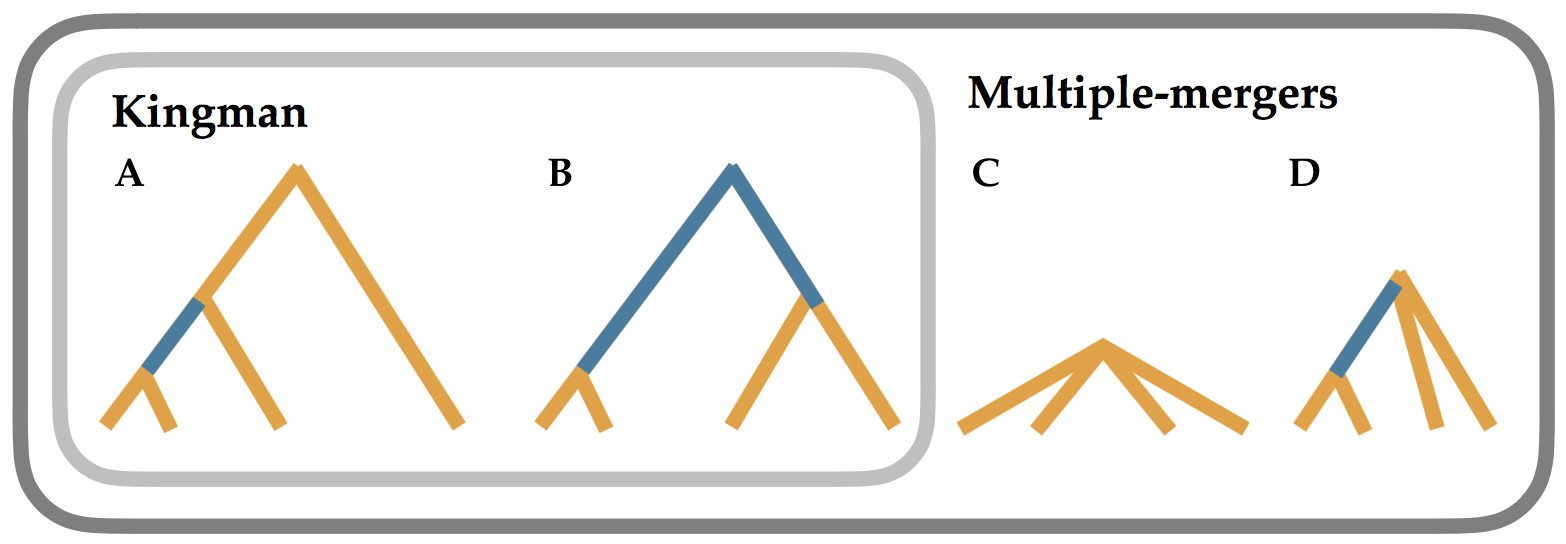
\includegraphics[width=0.8\textwidth]{figures/trees.png}
\caption{Possible genealogies with a sample size of $n=4$. Opportunities for singleton/tripleton mutations are in orange. Opportunities for doubletons are in blue.  \label{fig:trees}}
\end{figure}

We can get an intuitive understanding for this result by considering a sample of size 4. In the Kingman coalescent, there are only two possible tree topologies (\Fig{fig:trees}).
Furthermore, the total branch length is independent of the topology.
As a result, there is a trade-off between the branch length leading to singleton/tripleton mutations and the branch length leading to doubletons: loci with topology (A) will have more opportunities for the former and loci with topology (B) will have more opportunities for the latter.
Conditional on observing a doubleton at a locus, it is thus more likely that the locus has topology (B) and so the expected number of singletons is lower.
In terms of the joint site frequency spectrum, we have $\E{\phi_{12}} < \E{\phi_{1}} \E{\phi_{2}}$.

On the other hand, multiple mergers induce correlations between the tree topology and the total branch length.
For example, topology (C) has less overall opportunity for singletons as well as doubletons than (A) or (B), even though the expected proportion of singletons is higher.
Thus, observing \emph{any mutation at all} makes topology (C) less likely and the expected number of other mutations at all frequencies more likely.
If multiple-mergers events are frequent enough, this effect may dominate the tradeoff between (A) and (B) and lead to $\E{\phi_{12}} > \E{\phi_{1}} \E{\phi_{2}}$.

There are two limitations of these existing results.
First, they only apply to time-homogeneous coalescent processes and thus do not distinguish between multiple-mergers coalescents and Kingman models with time-varying population size.
Second, they assume a non-recombining locus and may break down for sites separated by a finite genetic distance.

\subsubsection{Weakly-linked sites}

Previous work on the multiple-mergers coalescent with recombination is limited relative to the literature on multiple-mergers models in non-recombining loci.
Nonetheless, existing results suggest that the two-site joint site frequency spectrum will behave differently as a function of genetic distance in multiple-mergers versus Kingman models.

Eldon and Wakeley \cite{} calculated the expected linkage disequilibrium (LD) in a modified Wright-Fisher model with occasional ``jackpot'' reproductive events.
In these events, one individual is selected to be the ancestor of a fixed finite fraction of the population.
As a result, even in the $N \to \infty$ limit, more than two lineages may share the same ancestor in the same generation.
Eldon and Wakeley found that LD may be reduced by multiple mergers at short genetic distances because of the elevated proportion of singleton mutations in this model.
This effect is similar to the impact of population growth on LD.
In contrast, the authors found that pairwise coalescent times at two unlinked sites may be correlated due to jackpot events: there is a finite probability that both lineages at both sites are descended from the ``lucky'' ancestor.

Birkner et al. \cite{} extended the results of Eldon and Wakeley \cite{} by deriving the ancestral recombination graph for a diploid population with jackpot reproductive events.
They show that in this model, the limiting marginal coalescent process is a simultaneous multiple-mergers coalescent with up to four simultaneous mergers permitted.
(The four possible mergers are due to the four chromosomes of the two diploid parents of the jackpot event.)
Birkner et al. found that the correlations in pairwise coalescent times found by Eldon and Wakeley holds for correlations between coalescent times in samples larger than two.
This results suggests that the two-site frequency spectrum considered as a function of genetic distance will be informative for identifying multiple-mergers coalescent processes. 

\section{Methods}

\subsection{Summary statistics}

We would like to detect signals of non-Kingman coalescent processes in polymorphism data from a sample of size $n$ where the ancestral state is unknown.
Thus, we will calculate statistics of the expected \textit{folded} site frequency spectrum, $\E{\eta_i }= \E{\phi_i + \phi_{n-i}}$, which is symmetric under the exchange of the ancestral and derived alleles.
This quantity is the fraction of all sites (not only polymorphic sites) with minor allele frequency $i \in \{0, \ldots, \left \lfloor{n/2}\right \rfloor  \}$, and can be considered as a probability distribution.
We can therefore think of the folded two-site frequency spectrum as a joint probability mass function, $\E{\eta_{ij}}$ over  $\{0, \ldots, \left \lfloor{n/2}\right \rfloor  \}^2$, the set of minor allele frequencies at the left and right positions.

We are interested in the signatures of genealogical distortions that affect the two-site frequency spectrum beyond their effects on the single-site frequency spectrum.
A natural transformation of the data is the pointwise mutual information:
\begin{equation}
\pmi(i,j) = \log_2 \left( \frac{\E{\eta_{ij}}}{\E{\eta_i} \E{\eta_j}} \right).
\label{eq:pmi}
\end{equation}
Pointwise mutual information is a commonly-used measure of the strength of relationship between two random variables and is equal to the log ratio of the joint probability to the product of the marginal probabilities.
(The more familiar mutual information is equal to the expectation of the pointwise mutual information.)
An advantage of the pointwise mutual information in our setting is that for $i,j \geq 1$ both the numerator and denominator in \eq{eq:pmi} scale like $(T_2 \mu)^2$, so that PMI is insensitive to the mutation rate and pairwise coalescent time, and only measures the shapes of genealogies.

In order to highlight the portions of the joint site frequency spectrum that are most salient and easiest to estimate from finite data, we will also calculate the weighted pointwise mutual information:
\begin{equation}
\wpmi(i,j) = \frac{\E{\eta_{ij}}}{\bar{\pi}^2} \log_2 \left( \frac{\E{\eta_{ij}}}{\E{\eta_i} \E{\eta_j}} \right),
\label{eq:pmi}
\end{equation}
for $i, j \geq 1$, where $\bar{\pi} = 2T_2 \mu$ is the average pairwise diversity and preserves the invariance to changes in mutation rate.

\subsection{Simulations}

For time-homogeneous $\Lambda$-coalescents without recombination, the expected joint site frequency spectrum may be calculated numerically using the recursion in \cite{birkner:etal:2013}.
However, this algorithm is $\mathcal{O}(n^4)$ in the size of the sample and is thus impractical to calculate for large samples.
Furthermore, there are no analytical results for recombining loci, time-varying coalescent rates, or models with natural selectuion.
We therefore turn to simulations.

We ran coalescent simulations using a version of the program \texttt{msprime} \cite{msprime} modified to allow for multiple-mergers according to the Beta coalescent model.
[NOTE: it probably would not be too complicated to also do simultaneous multiple-mergers as suggested by Matthias Steinrucken.]
Because we are interested in summary statistics that are independent of the rate of neutral mutations, we run the coalescent simulations without mutations and calculate expected site frequency spectra directly from branch lengths.
This approach allows us to extract the maximum amount of information from each simulation run.

We are primarily interested in distinguishing multiple-mergers coalescents from Kingman coalescent models of growing populations because these models generate similar single-site frequency spectra.
First, we consider a growing population where the population size (inverse coalescence rate) is given by
\begin{equation} N(t) = N_0 \exp (- gt),\end{equation}
 where $t$ is the time before the present.
In this model, the control parameter is $gN_0$, the population growth rate in coalescent time units.
[NOTE: I could also use a model where the population was constant up until a time $T_g$ in the past and then began to grow exponentially. I suspect this won't change anything except adding another parameter, but I probably should test it out in at least a few cases.]

Recent evidence suggests that some populations, including humans, may be growing at a faster-than-exponential rate \cite{} and that such growth may distort genealogies \cite{}.
As a model for faster-than-exponential growth, we simulate piecewise-constant population sizes with two epochs:
\begin{equation}
N(t) = 
\begin{cases}
      N_0, &  t < T_g \\
      N_0 / \gamma, & t \geq T_g.
\end{cases}
\end{equation}
Patterns of diversity in this model are determined by $T_g / N$, the time of the growth, in coalescent units and $\gamma > 1$, the instantaneous growth factor.

For simulations of recombining loci, we varied $r$, the per-generation recombination rate between the focal positions.
These simulations have an additional control parameter $rT_2$, where $T_2$ is the average pairwise coalescent time measured from the simulations.

[TO-DO: I've implemented bottleneck, 2-deme, and many-deme stepping-stone population simulations, but need to re-run them with the current approach.]

[TO-DO: Simulations of linked-selection using SLiM \cite{slim:paper}. It's installed on the cluster and locally. I've learned how use it and run a few tests. I need to pick parameter values and run simulations at scale.] 

\subsection{Data analysis}

\subsubsection{Zambian \textit{Drosophila melanogaster}}

We calculated the 2-site frequency spectrum of single nucleotide polymorphisms in a sample of whole genome sequences ($\sim40x$ coverage) of $\sim200$ \textit{Drosophila melanogaster} from Zambia \cite{}.
This population is believed to be from the ancestral range of the species, is very diverse ($\pi \approx 1\%$), and has limited global admixture \cite{}.
We downloaded the individual consensus sequences available from the Drosophila Genome Nexus at \url{http://www.johnpool.net/genomes.html}, removed chromosome arms with known inversions, and downsampled to one hundred samples for each chromosome arm.
In order to focus on high-quality sites and to simplify the interpretation of the allele frequency spectrum, we considered only sites with confident genotypes called in all one hundred samples (XX\% of sites.)
[TO-DO: Look at only 4-fold degenerate sites. I've already identified them]

To estimate the recombination rate between sites, we used the recombination map published by Comeron \textit{et al.} \cite{}, and available at \url{https://petrov.stanford.edu/cgi-bin/recombination-rates_updateR5.pl}.
This map has a resolution of 100KB and was calculated by identifying individual cross-over events in XX trios.
While the scale of this experiment was immense, the average number of observed cross-over events per window was only XX and so much of the window-to-window variation appears to be attributable to counting noise.
To reduce the effect of this noise, we applied a standard wavelet de-noising procedure \cite{} to the recombination rate as a function of genomic position, yielding a smoother map [refer to an appendix].
This recombination map yields a stronger relationship between recombination rate and diversity than the original map, a well-known feature of the \textit{D. melanogaster} genome \cite{begun:aquadro, etc}, suggesting that the wavelet de-noising was successful.

\subsubsection{European humans}
[TO-DO: EVE consortium European humans. deCODE genetic map]

\section{Results}

\subsection{Simulations}
\Fig{fig:msfs} shows the average single-site frequency spectra for calculated from coalescent simulations as described above.
Time-homogeneous Beta coalescent simulations range from the Kingman coalescent ($\alpha=2$) through increasing intensities of multiple-mergers as $\alpha \to 1$.
(The $\alpha  \to 1$ limit is the Bolthausen-Sznitman coalescent.)
The site frequency spectrum shows an excess of rare alleles relative to the Kingman expectation, and this excess is stronger for smaller values of $\alpha$.

As expected, Kingman coalescent simulations of growing populations also show an excess of rare alleles.
This distortion is more extreme for larger growth rates and the precise shape of the site frequency spectrum depends on the growth rate or timing of instantaneous growth.
Note that our goal here is not to find population growth models that precisely reproduce the site frequency spectra of Beta coalescents, but to show that the qualitative behavior of the two classes of models is similar.

\begin{figure}
\centering
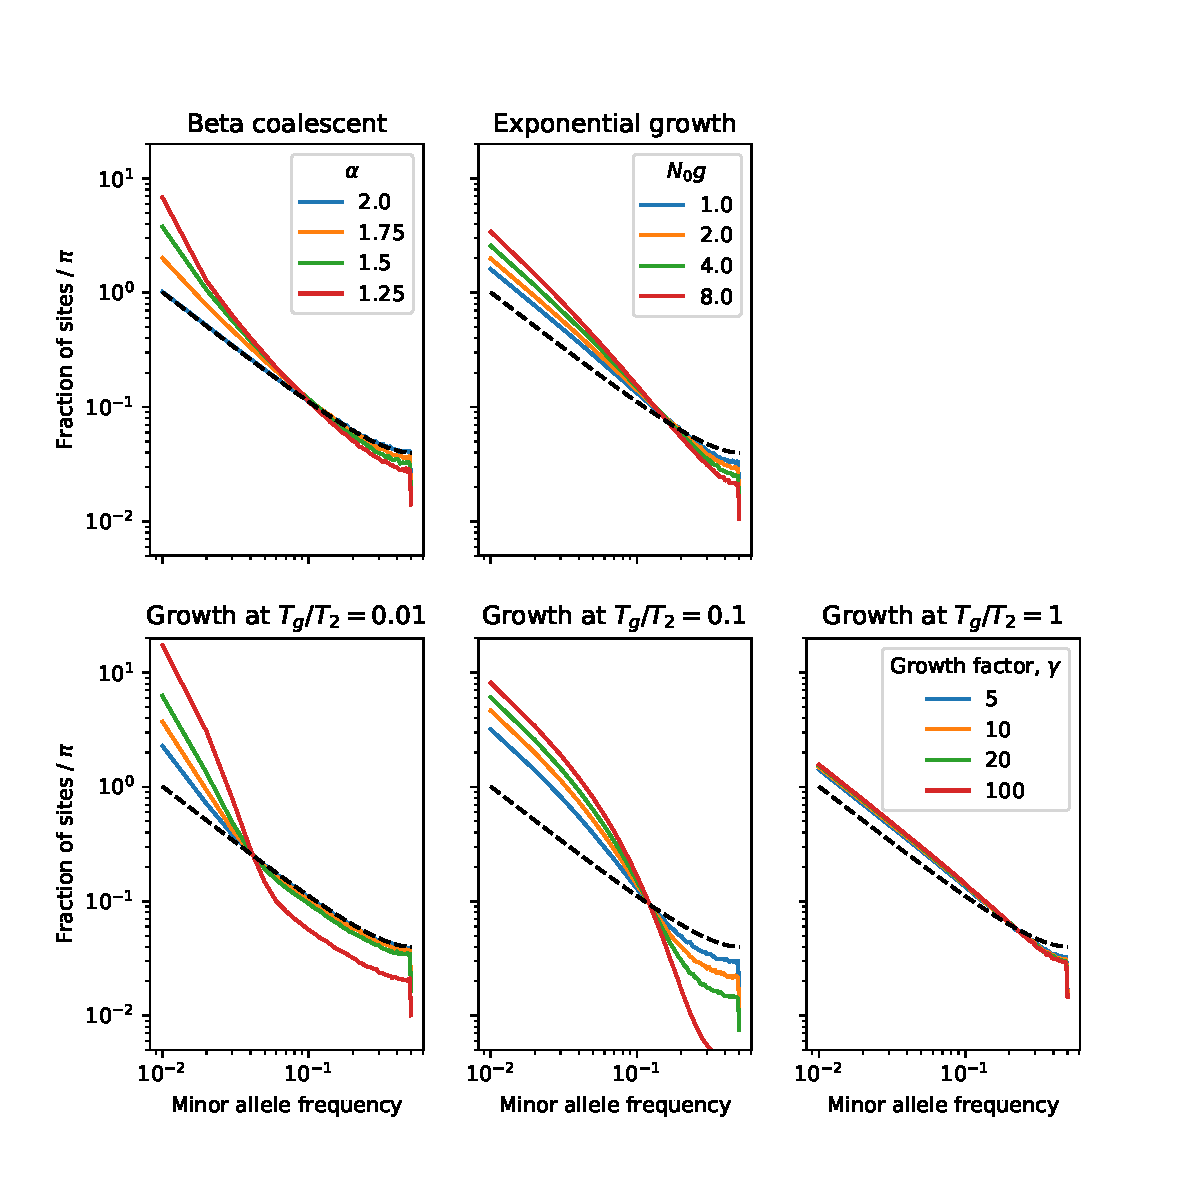
\includegraphics[width=0.8\textwidth]{figures/mSFS.pdf}
\caption{The single-site frequency spectrum compared to time-homogeneous Kingman expectation (dashed line) for multiple-mergers (Beta) coalescent, exponentially-growing populations, and instantaneously-growing populations (bottom row) as described in Methods. Spectra are normalized by the average pairwise diversity $\pi$.  \label{fig:msfs}}
\end{figure}

\subsubsection{Two-site frequency spectra of non-recombining loci}

\begin{figure}
\centering
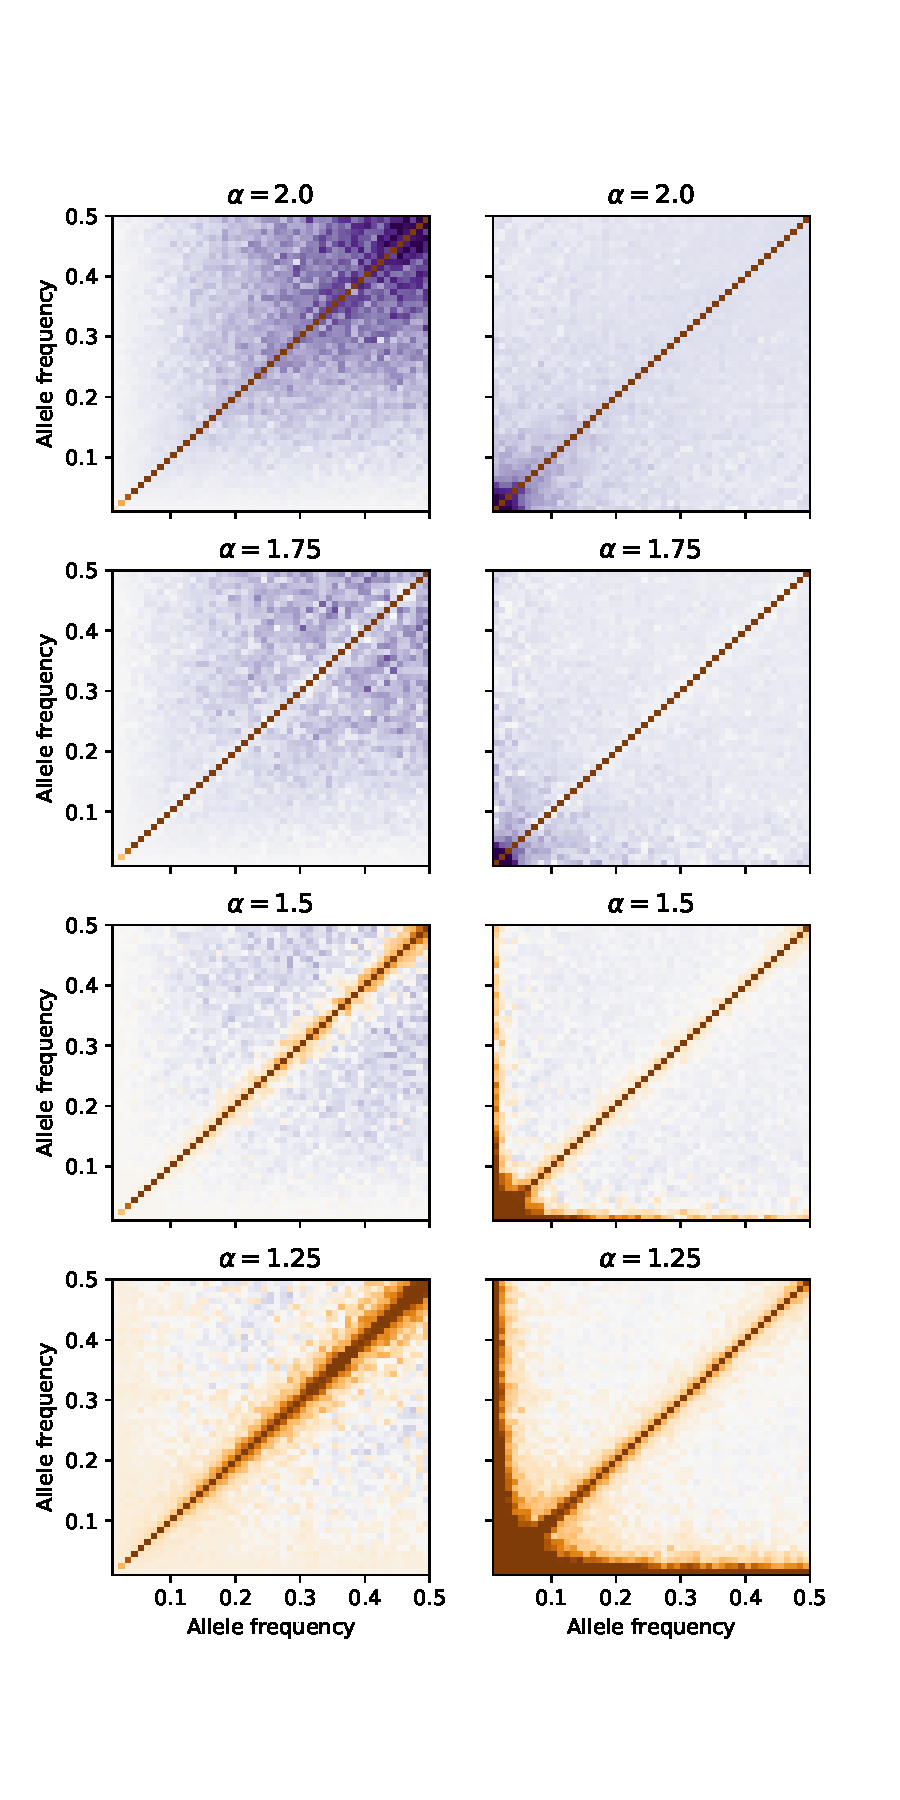
\includegraphics[width=0.6\textwidth]{figures/pmi_beta_r0.pdf}
\caption{PMI (left) and wPMI (right) for time-homogeneous Beta coalescent simulations without recombination. Positive values are in orange, negative values are in purple. [TODO: colorbar]\label{fig:pmi_beta_r0}}
\end{figure}

\Fig{fig:pmi_beta_r0} shows the pointwise mutual information and weighted pointwise mutual information for time-homogeneous Beta coalescent simulations without recombination.
As expected, the Kingman coalescent has only negative values away from the diagonal, while increasing the intensity of multiple mergers leads to positive off-diagonal values.
In particular, multiple mergers induce positive correlations between the numbers of alleles at similar but not identical frequencies, as shown by the positive values near the diagonals.
Finally, the weighted pointwise information reveals that multiple mergers lead to positive correlations between the numbers of low-frequency and high-frequency mutations at linked sites.

\begin{figure}
\centering
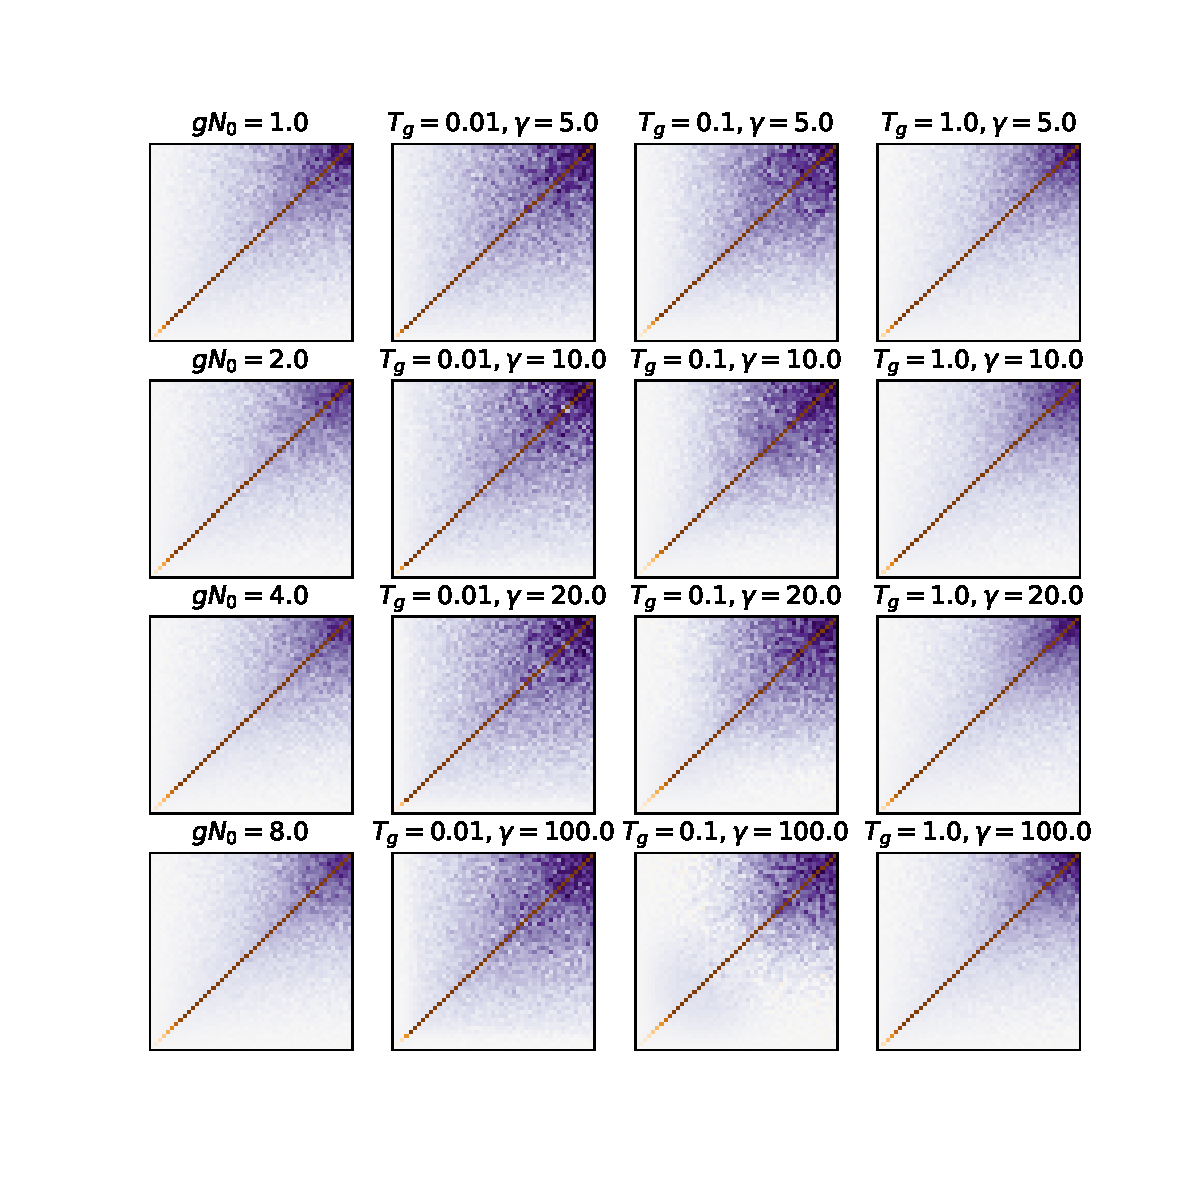
\includegraphics[width=\textwidth]{figures/pmi_growth_r0.pdf}
\caption{PMI in Kingman coalescent simulations of growing populations without recombination. Left column shows exponential growth. Other columns show instantaneous growth. Positive values are in orange, negative values are in purple. [TODO: colorbar]\label{fig:pmi_growth_r0}}
\end{figure}

\begin{figure}
\centering
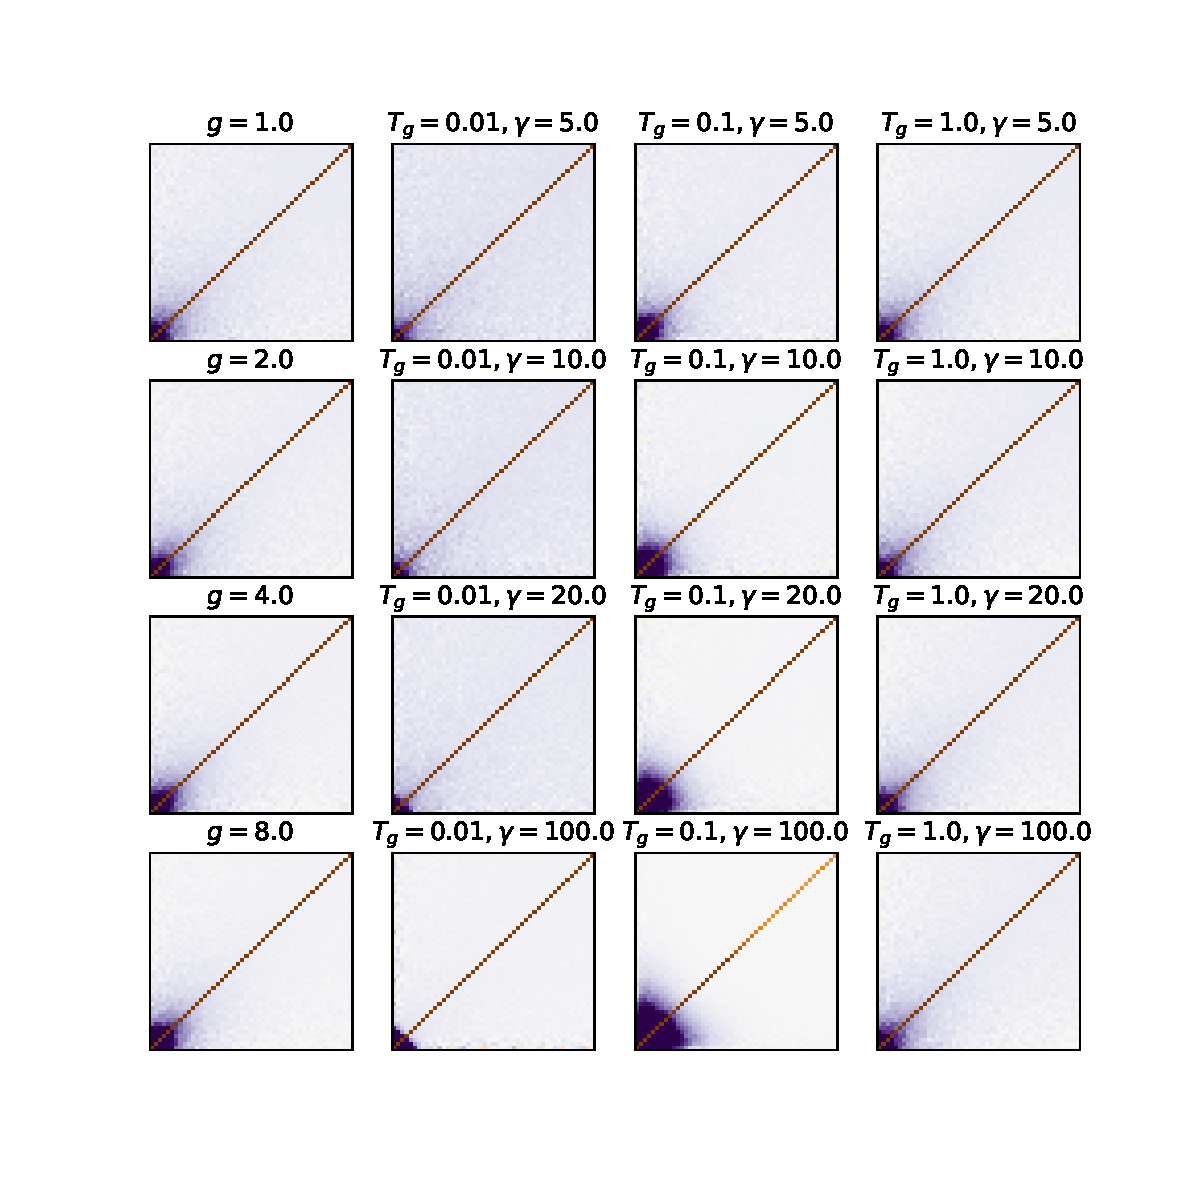
\includegraphics[width=\textwidth]{figures/wpmi_growth_r0.pdf}
\caption{wPMI in Kingman coalescent simulations of growing populations without recombination. Left column shows exponential growth. Other columns show instantaneous growth. Positive values are in orange, negative values are in purple. [TODO: colorbar]\label{fig:wpmi_growth_r0}}
\end{figure}

\Fig{fig:pmi_growth_r0} and \Fig{fig:wpmi_growth_r0} show the pointwise mutual information and weighted pointwise mutual information respectively for models of population growth without recombination.
Together they show that, unlike the single-site frequency spectrum, these transformations of the two-site frequency spectrum of linked sites are relatively insensitive to population growth.
All of the parameters considered generate PMI values that are negative for alleles at different frequencies.
This suggests that the two-site frequency spectrum contains information that can qualitatively distinguish between Kingman and multiple-mergers coalescent processes.

\subsubsection{Two-site frequency spectra of recombining loci}

\begin{figure}
\centering
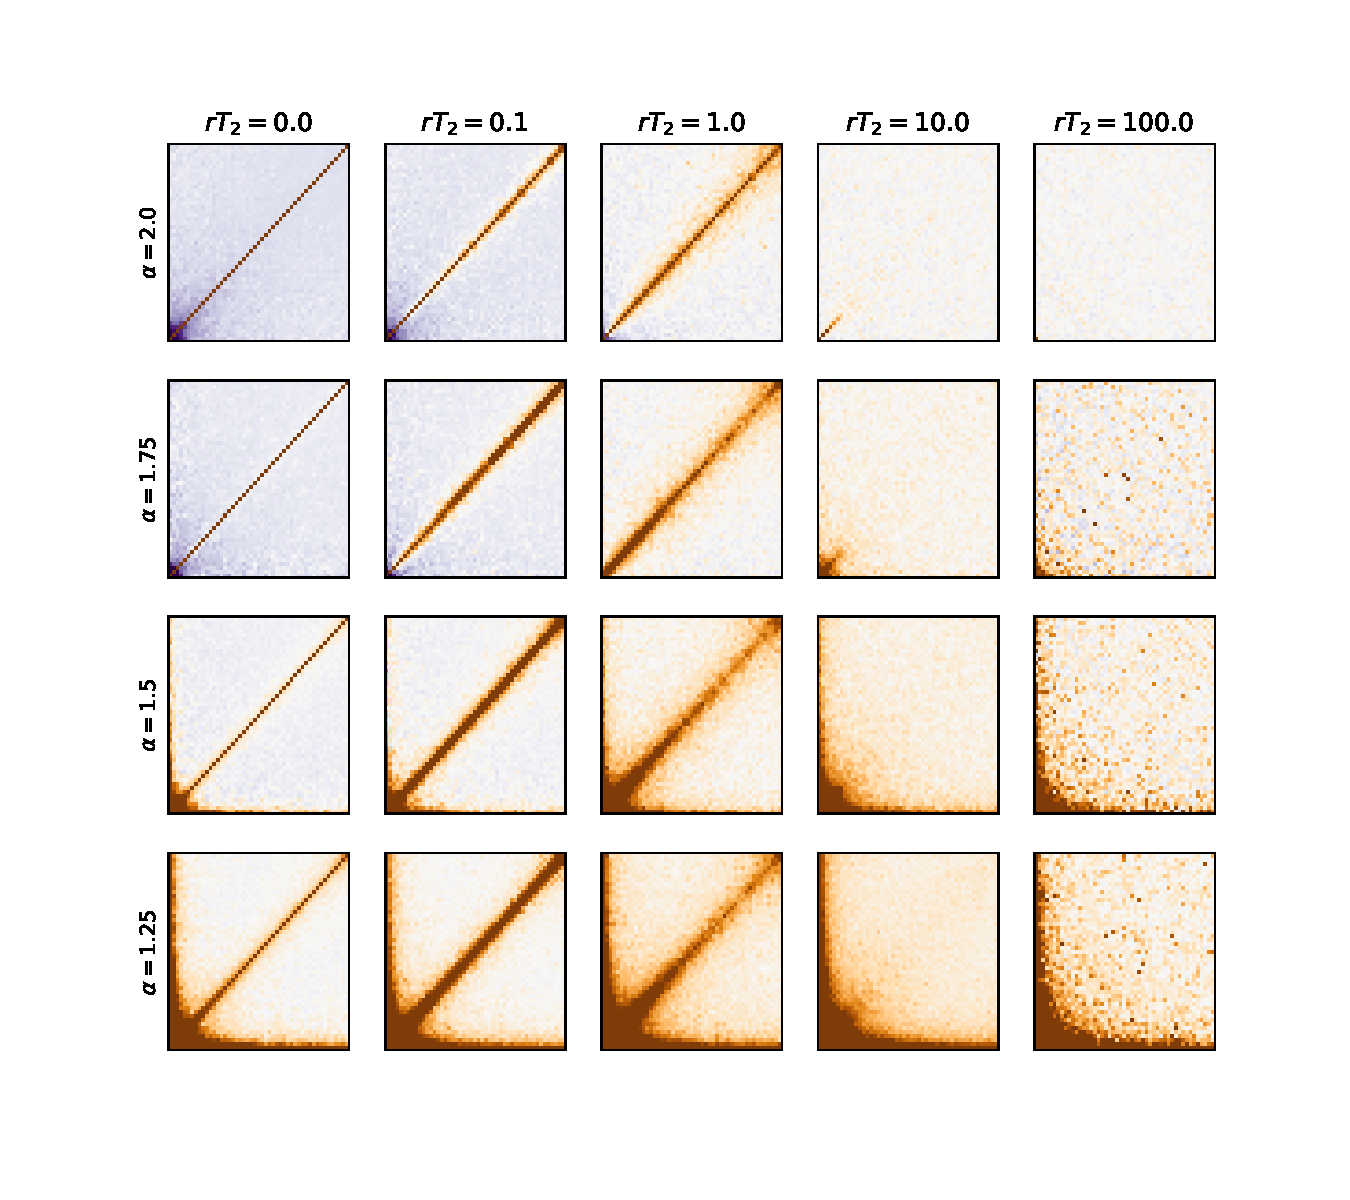
\includegraphics[width=\textwidth]{figures/wpmi_beta_r.pdf}
\caption{wPMI in Beta coalescent simulations of loci with recombination. Positive values are in orange, negative values are in purple. [TODO: colorbar]\label{fig:wpmi_beta_r}}
\end{figure}

\Fig{fig:wpmi_beta_r} shows the weighted pointwise mutual information for time-homogeneous Beta coalescent simulations with recombination.
The beta coalescent simulations have overall more positive PMI values than the Kingman coalescent at all recombination rates
On the other hand, at intermediate recombination rates $rT_2 \sim 1$, the Kingman simulations have positive associations between alleles at similar frequencies, muddying this feature as a signature of multiple mergers.
(These positive correlations are due to the partial breakdown of size-$i$ clades into size-$i-\delta_i$ clades at moderately-linked sites.)

However, there are two signals that appear to be robust to recombination.
First, the positive association between low-frequency and high-frequency alleles is not present in the Kingman simulations at any recombination rate.
Second, this positive association persists even at large genetic distances in the Beta coalescent simulations.
In contrast, in the Kingman simulations, all mutual information between the two sites decays to zero at genetic distances greater than $rT_2 \sim 1$.

\begin{figure}
\centering
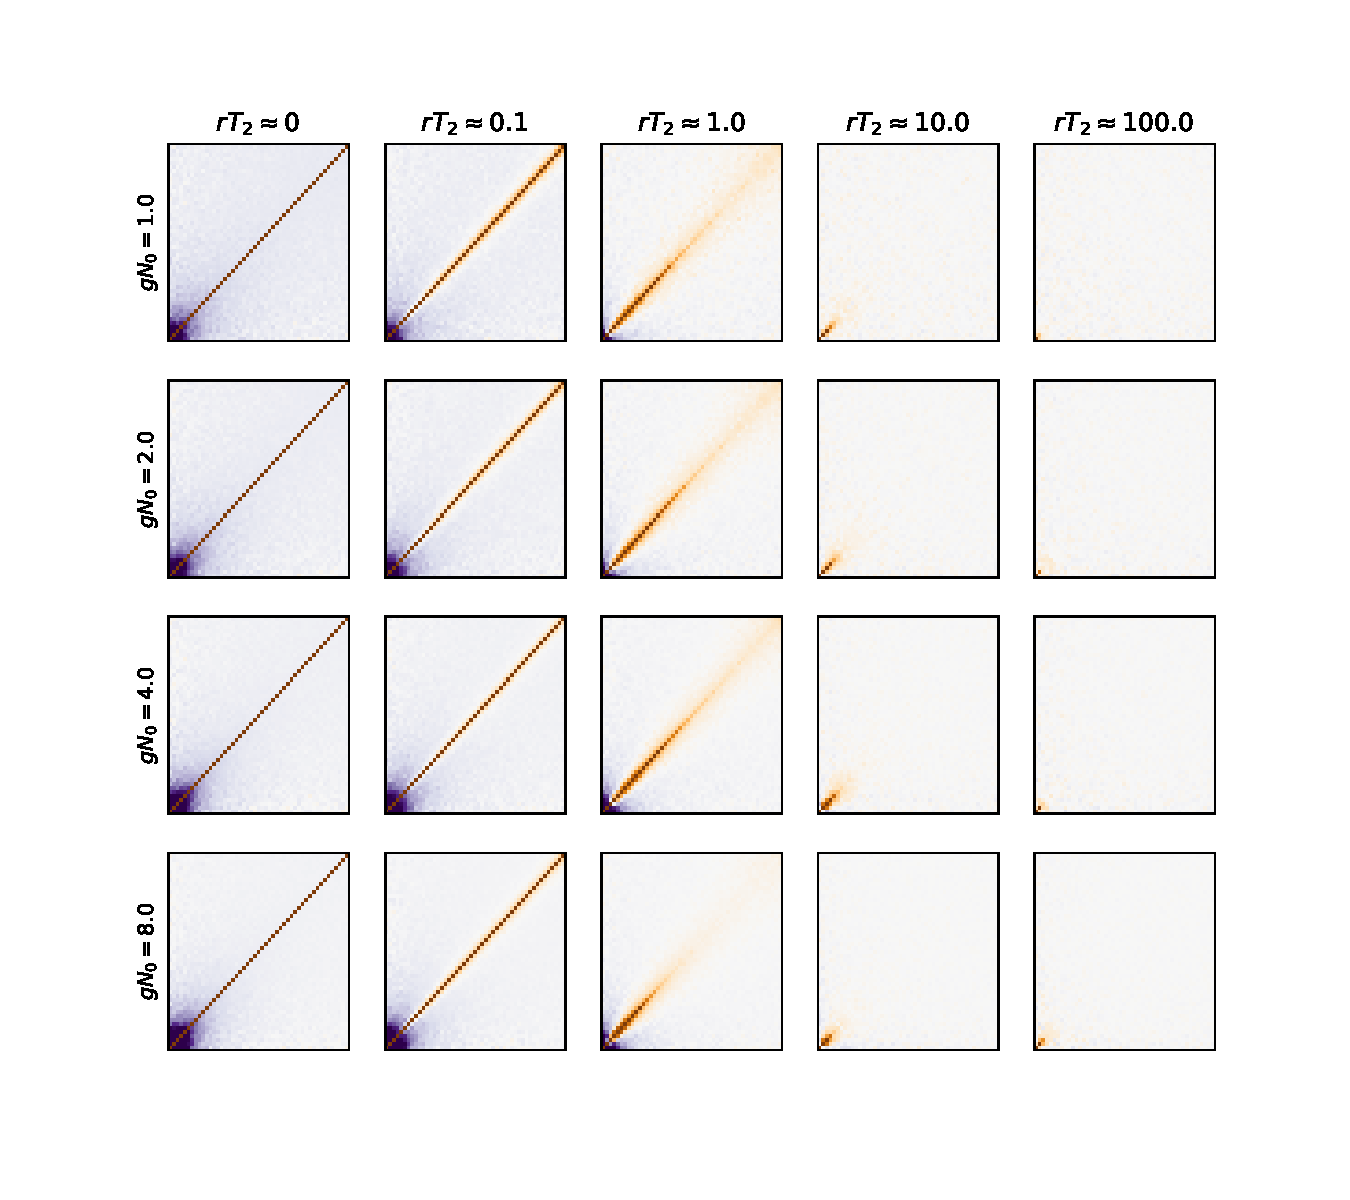
\includegraphics[width=\textwidth]{figures/wpmi_exp_r.pdf}
\caption{wPMI in Kingman coalescent simulations of exponential growth with recombination. Positive values are in orange, negative values are in purple. [TODO: colorbar]\label{fig:wpmi_exp_r}}
\end{figure}

\begin{figure}
\centering
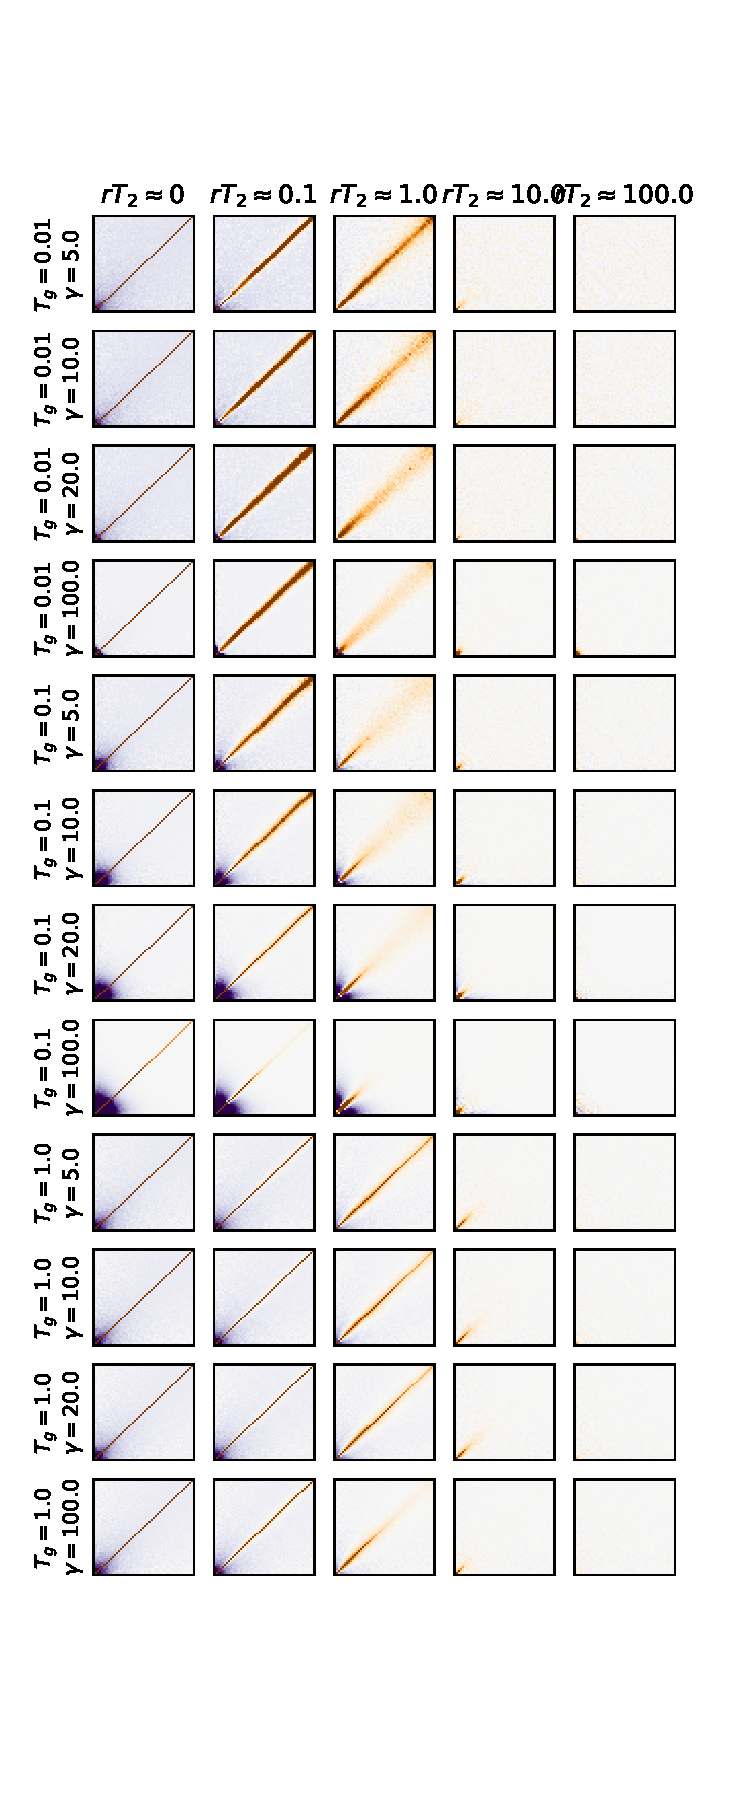
\includegraphics[width=.6\textwidth]{figures/wpmi_step_r.pdf}
\caption{wPMI in Kingman coalescent simulations of instantaneous growth with recombination. Positive values are in orange, negative values are in purple. [TODO: colorbar]\label{fig:wpmi_step_r}}
\end{figure}

\Fig{fig:wpmi_exp_r} and \Fig{fig:wpmi_step_r} show the weighted pointwise mutual information for models of population growth without recombination.
While the different results vary in detail, they all share the same key features with the time-homogeneous Kingman model:
(1) recombination generates positive associations between alleles at similar frequencies, but not between high- and low-frequency alleles, and
(2) mutual information decays to zero for $rT_2 \gg 1$.

These simulation results suggest a simple new data summary that can qualitatively distinguish between genealogical distortions due to multiple mergers and those due to population growth.
We reduce the site frequency spectrum to two elements by defining the expected non-singleton frequency:
\begin{equation}
\E{\eta_{>1}} = \sum_{i=2}^{\left \lfloor n/2 \right \rfloor} \E{\eta_i},
\end{equation}
and similarly define the reduced two-site frequency spectrum.
The association between high- and low- frequency alleles is captured by the pointwise mutual information between singletons and non-singletons:
\begin{equation}
\log_2 \left( \frac{\E{\eta_{1,>1}}}{\E{\eta_1} \E{\eta_{>1}}} \right).
\label{eq:singleton_pmi}
\end{equation}

\begin{figure}
\centering
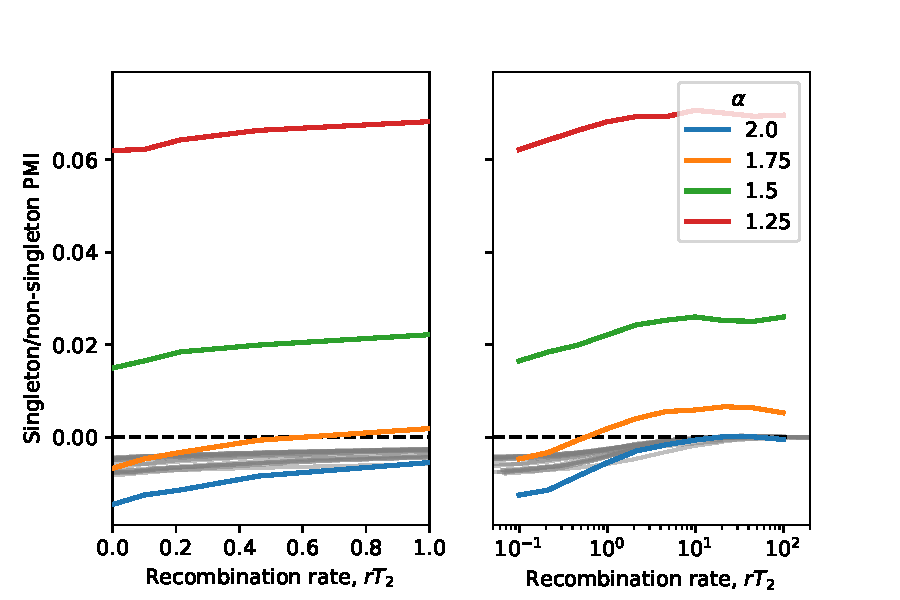
\includegraphics[width=\textwidth]{figures/singleton_pmi_all.pdf}
\caption{Singleton/non-singleton PMI in all coalescent simulations recombination. Colored curves show time-homogeneous Beta coalescent (including Kingman in blue.) Grey curves show all population growth simulations. \label{fig:singleton_pmi}}
\end{figure}

\Fig{fig:singleton_pmi} shows \eq{eq:singleton_pmi} for all simulations.
The left panel shows that, for each coalescent process, the singleton/non-singleton PMI is not very different between perfectly loci, $rT_c=0$, and moderately-linked loci $rT_c \sim 1$.
The right panel shows that singleton/non-singleton PMI decays to zero at long genetic distances for Kingman models, but not the Beta coalescent. 
At no point do any of the Kingman coalescent models generate positive singleton/non-singleton PMI.

\subsection{Data analysis}

\subsubsection{Zambian \textit{Drosophila melanogaster}}
\begin{figure}
\centering
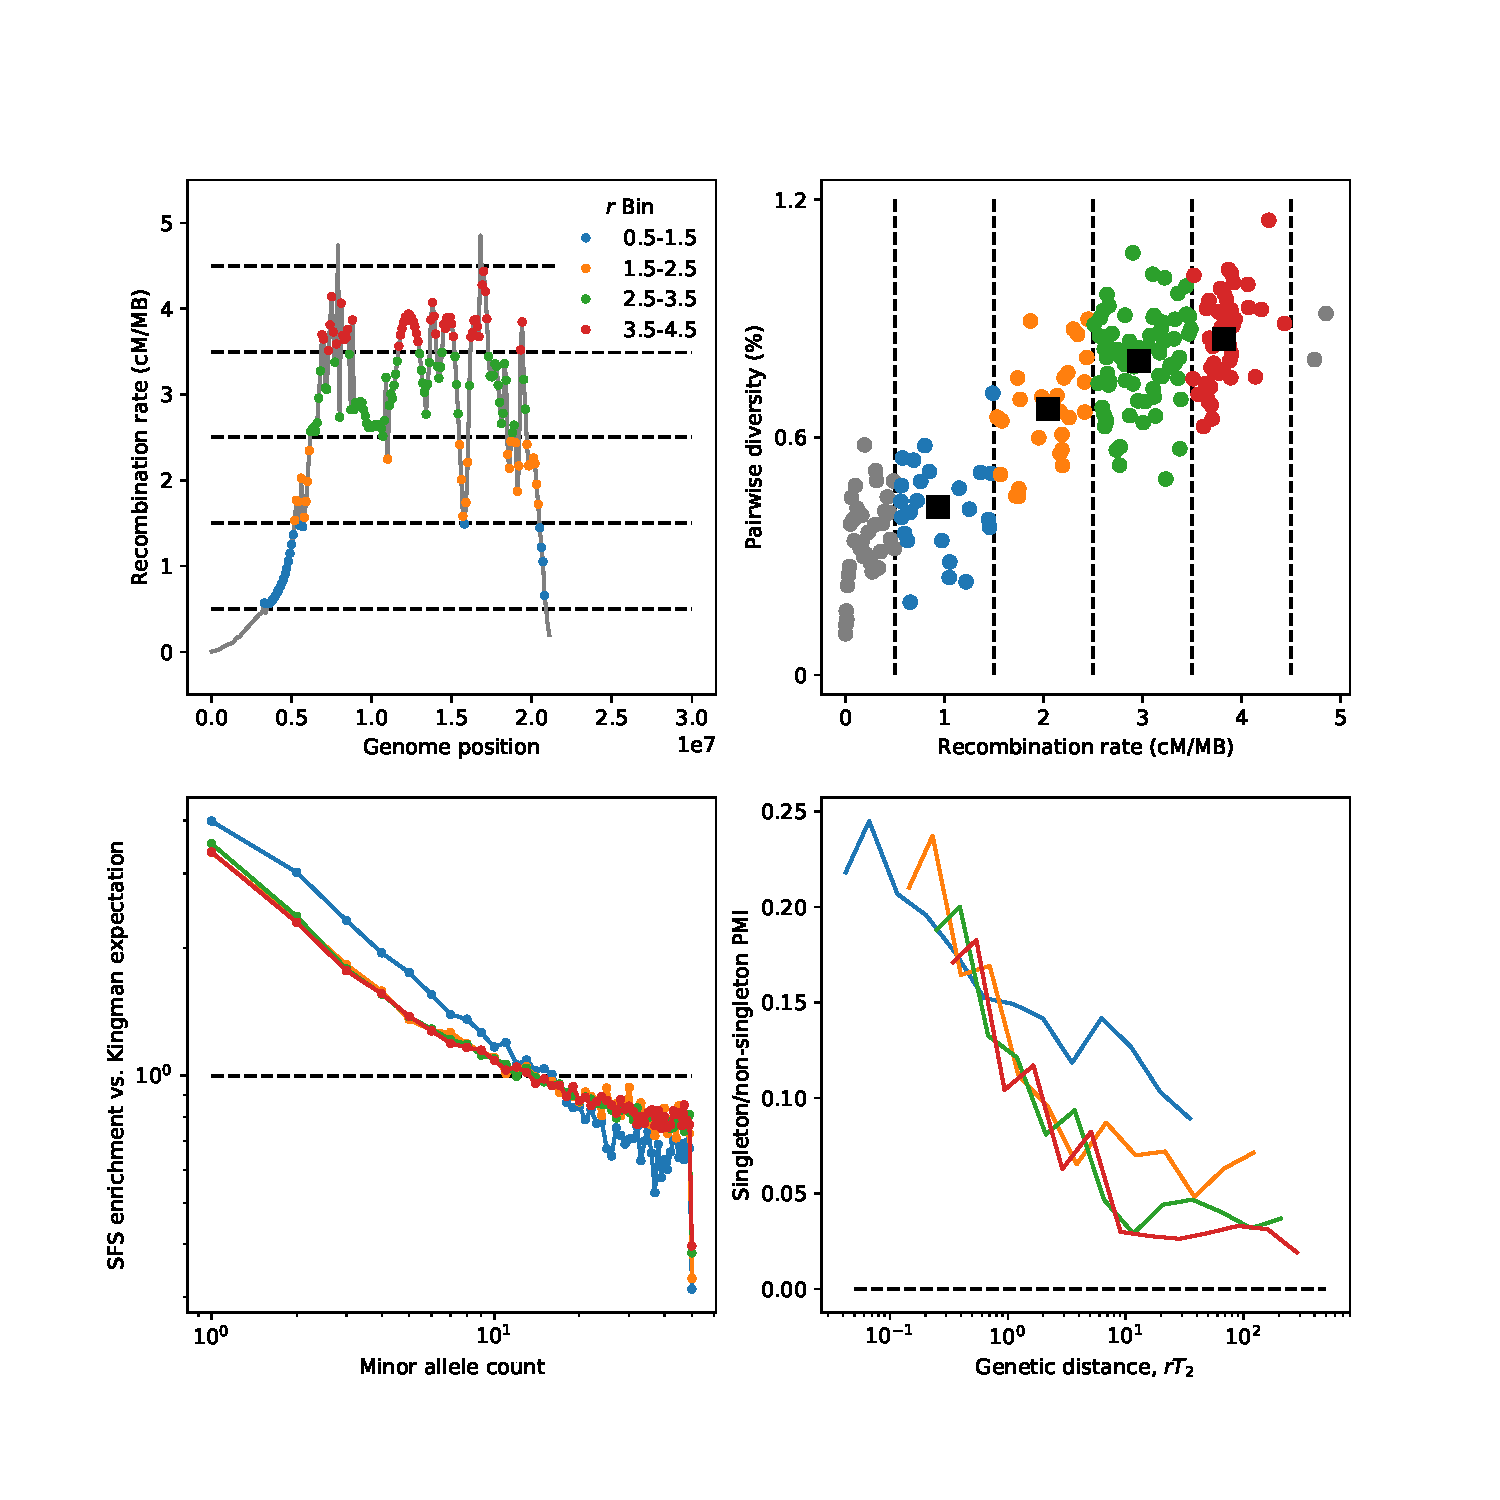
\includegraphics[width=\textwidth]{figures/chr2R_summary.pdf}
\caption{\textit{Drosophila} chromosome arm 2R summary. (A) Recombination rate in 100kb windows. We grouped the data into four evenly-spaced bins by recombination rate (colors). (B) Average pairwise diversity is higher in bins with higher recombination rate. (C) All recombination-rate bins show an excess of low-frequency alleles relative to the Kingman expectation. The lowest-recombination bin shows the most distortion. (D) Singleton/non-singleton PMI is positive and persists at long genetic distances. \label{fig:drosophila}}
\end{figure}

We partitioned chromosome arm 2R into four bins by our de-noised estimates of the recombination rate in 100KB windows (\fig{fig:drosophila}A, see methods).
The local recombination rate is a good predictor of the local average pairwise diversity, as has been shown before for \emph{D. melanogaster} (\fig{fig:drosophila}B).
This relationship is putatively due to the action of background selection or selective sweeps \cite{}.
If this hypothesis is correct, we expect to see more signatures of non-Kingman coalescent processes in the regions of low recombination.
In fact, we see that the single-site frequency spectrum deviates from the time-homogeneous Kingman expectation in all windows, but especially in the lowest-recombination window (\fig{fig:drosophila}C).
We also find positive singleton/non-singleton PMI in all windows (\fig{fig:drosophila}D).
Furthermore, this positive association does not decay to zero for $rT_2\gg1$, as expected from the multiple-mergers simulations.
This signal appears to be stronger in lower-recombination rate windows than in high-recombination rate windows.

On the other hand, the decay of singleton/non-singleton PMI at short genetic distances ($rT_2<1$) is not predicted from our beta coalescent simulations.
[Is this because selection generates different ARGs from $\Lambda$-coalescents? Is it because of some genomic property or data artifact we're not modeling?]

[TO-DO: Alternative explanations. e.g. variation in mutation rate]

[TO-DO: Other chromosome arms.]

[TO-DO: Replace binning by $r$ with something continuous.]

\subsubsection{European \textit{Homo sapiens}}
[TODO]

\end{document}

